\section{Methodology}\label{sec:Methodology}

\subsection{Problem Formulation}\label{sec:Methodology:formulation}

\textbf{Simplified Abstraction.} Without loss of generality, we consider a single prefill request processing through $L$ sequential Transformer layers. The communication workload for each layer can be generally abstracted as Multi-stage Flow (MsFlow). An MsFlow consists of three temporally dependent stages, where each stage constitutes a set of flow (or coflow) governed by the layer's lifecycle, which is detailed below:
\begin{enumerate}[label=$\bullet$,leftmargin=*,itemsep=0.5pt]
\item \textbf{Stage~1: Initialization.} Involves KV-cache reuse to transfer prerequisite states. This loosely coupled flow often overlaps with prior layer's computation to hide latency.
\item \textbf{Stage~2: Execution.} Consists of collective communication (e.g., alltoall) that strictly blocks the subsequent computation.
\item \textbf{Stage~3: Completion.} Handles the P2D transfer of results to decoding workers. This dictates the final token availability without blocking the current prefill computation.
\end{enumerate}

For a single request, MsFlows collectively share one TTFT deadline and may partially overlap subject to layer dependency (e.g., Stage~2 of layer $l$ must complete before computing layer $l+1$)

\textbf{Contention dynamics.} Contention arises when concurrent MsFlows compete for shared network bandwidth. Recall Fig~\ref{fig:bg:contention}, intra-request contention occurs between MsFlows of different layers within the same request, while inter-request contention arises between MsFlows of distinct requests. Both cases simply reduce to contention between heterogeneous stages.

\textbf{Overall Objective. } The goal is to meet end-to-end TTFT deadline (SLO attainment) rather than optimizing individual flow latencies. Specifically, we must orchestrate the dependent MsFlows to ensure that all $L$ MsFlows are completed within the deadline constraint. To achieve this, an ideal scheduler must balance two complementary objectives tailored to the specific semantics of MsFlow stages:
\begin{enumerate}[label=(\roman*),leftmargin=*,itemsep=0.5pt]
    \item \textbf{Minimizing Non-overlapped communication Latency.} For early stages (1\&2), completing too late directly prolongs the current layer's execution time, postponing the release of the subsequent layer.
    \item \textbf{Minimizing Earliness.} For the final Stage~3, completing too early yields no gain for meeting deadline but exacerbates potential network contention.
\end{enumerate}

\subsection{Key Observation and Scheduling Principle}
\begin{figure}[t!]
    \centering

    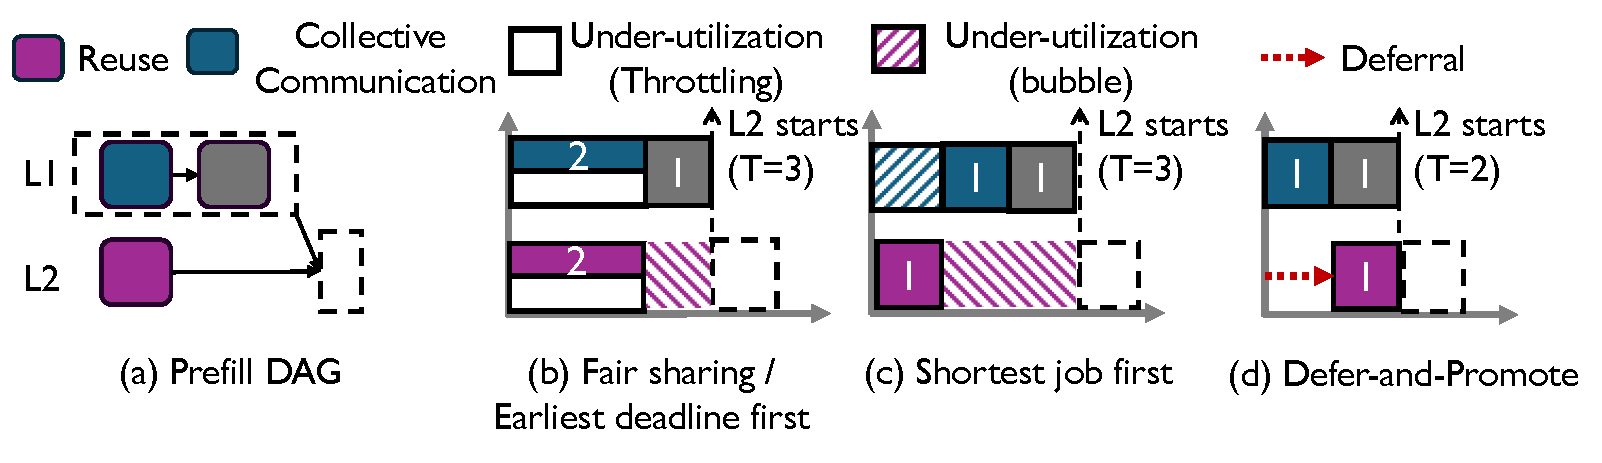
\includegraphics[width=\linewidth]{figures/methodology/IntraContentionExample-A.pdf}
    \caption{\textbf{Comparison of scheduling policies for intra-request contention (ingress).}
    (a) Ingress port contention during Layer-1 execution.
    (b)-(c) FS/SJF/EDF delays the start of Layer-2 ($T=3$).
    (d) The \textit{Defer-and-Promote} strategy advances the Layer-2 start time to $T=2$ (-33\%).}
    \label{fig:meth:intraA}

    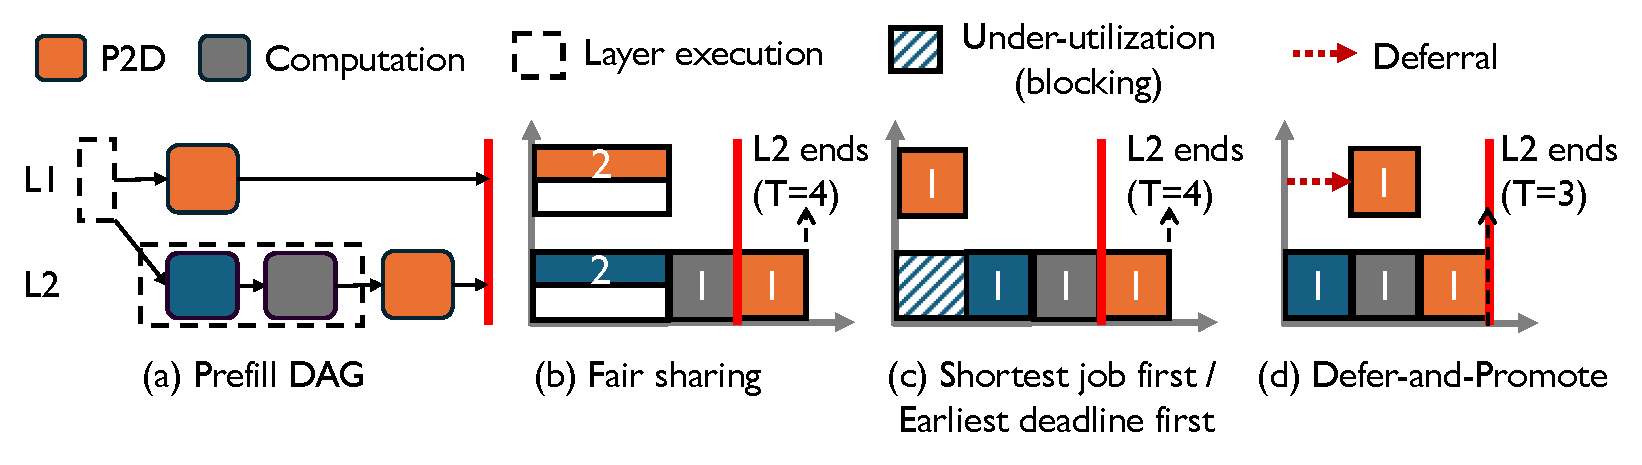
\includegraphics[width=\linewidth]{figures/methodology/IntraContentionExample-B.pdf}
    \caption{\textbf{Comparison of scheduling policies for intra-request contention (egress).}
    (a) Egress port contention during Layer-2 execution.
    (b)-(c) FS/SJF/EDF delays the end of Layer-2 ($T=4$).
    (d) The \textit{Defer-and-Promote} strategy reduces the Layer-2 finish time to $T=3$ (-25\%).}
    \label{fig:meth:intraB}
\end{figure}

\begin{figure}[t!]
    \centering

    \captionof{table}{An inter-request contention example.}
    \label{tab:InterReqExample}

    \fontsize{9}{11}\selectfont
    \begin{tabular}{c|c|c|c|c}
        \toprule
        \textbf{Req ID} & \textbf{Flow ID} & \textbf{Flow Size} & \textbf{Remain time} & \textbf{Deadline} \\
        \midrule
        1   & A & 2 & 9 & 18 \\
        2,3 & B & 4 & 6 & 12 \\
        4   & C & 3 & 0 & 7  \\
        \bottomrule
    \end{tabular}

    \begin{subfigure}{0.48\columnwidth}
        \centering
        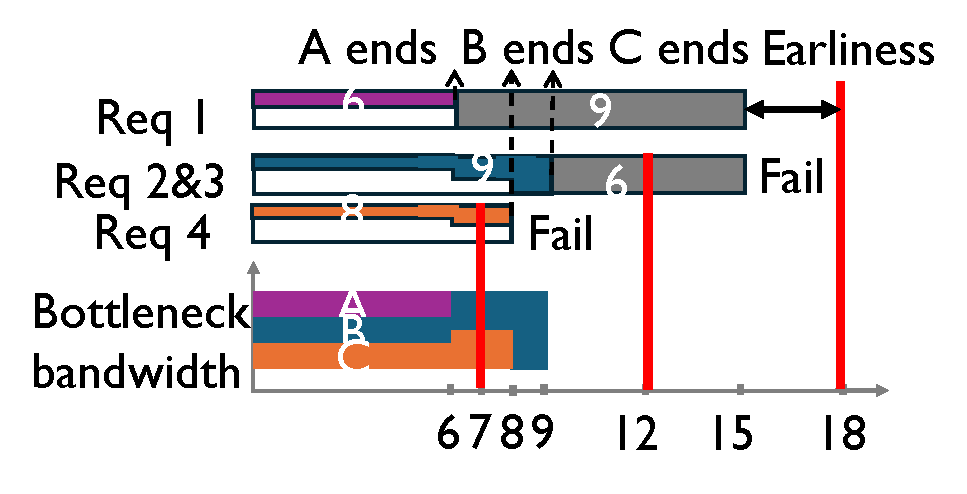
\includegraphics[width=\linewidth]{figures/methodology/InterContentionExample-FS.pdf}
        \caption{Fair Share}
        \label{fig:bg:expfs}
    \end{subfigure}
    \hfill
    \begin{subfigure}{0.48\columnwidth}
        \centering
        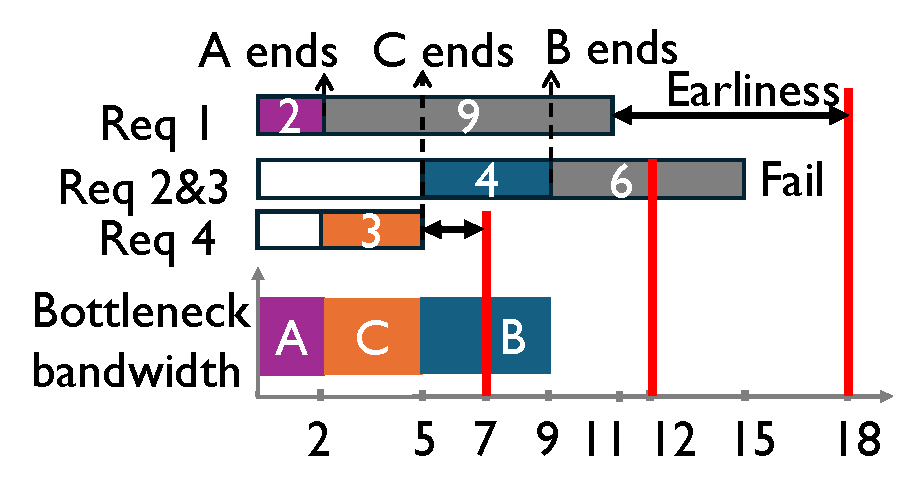
\includegraphics[width=\linewidth]{figures/methodology/InterContentionExample-SJF.pdf}
        \caption{Shortest Job First}
        \label{fig:bg:expsjf}
    \end{subfigure}

    \par\medskip

    \begin{subfigure}{0.48\columnwidth}
        \centering
        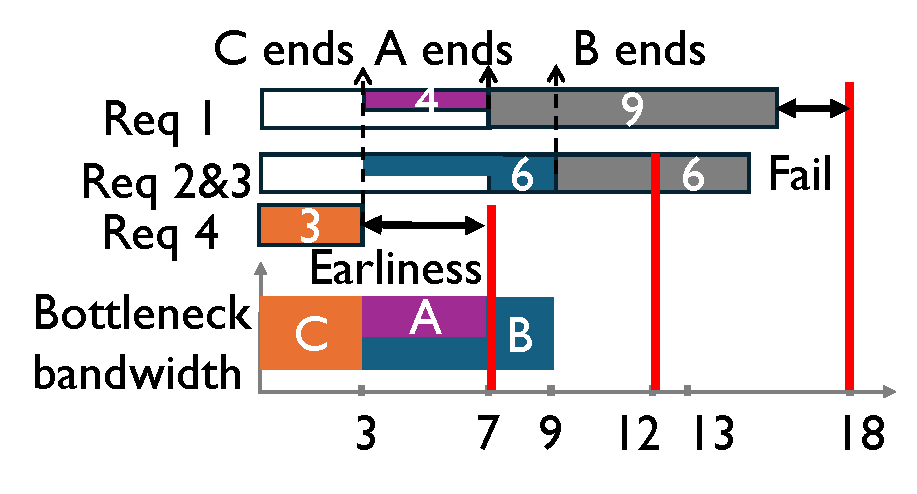
\includegraphics[width=\linewidth]{figures/methodology/InterContentionExample-EDF.pdf}
        \caption{Earliest Deadline First}
        \label{fig:bg:expedf}
    \end{subfigure}
    \hfill
    \begin{subfigure}{0.48\columnwidth}
        \centering
        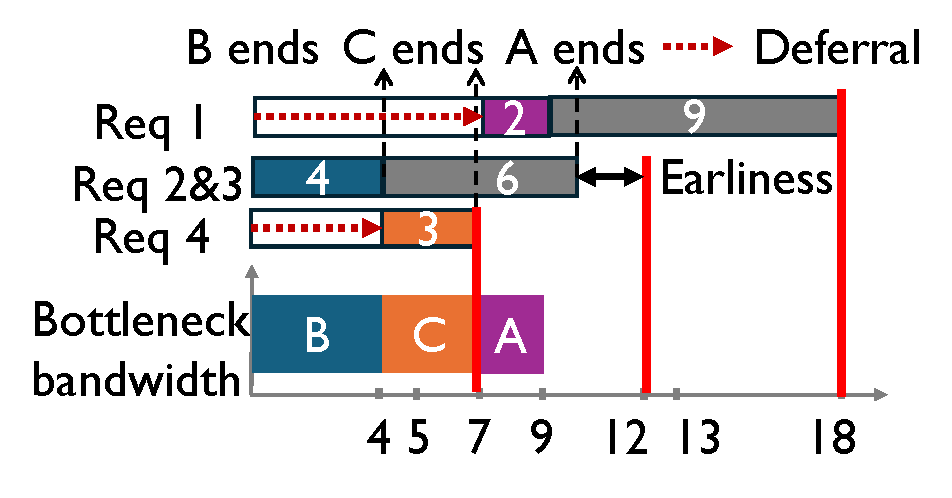
\includegraphics[width=\linewidth]{figures/methodology/InterContentionExample-DAP.pdf}
        \caption{Defer-and-Promote}
        \label{fig:bg:expopt}
    \end{subfigure}

    \caption{\textbf{Comparison of scheduling policies for inter-request contention.}
    The red vertical lines denote hard deadlines, and gray bars are subsequent durations.
    (a) Fair Share and (b) SJF fail to protect the urgent Flow-B due to lack of deadline awareness,
    while (c) EDF completes flows with explicit but loose deadlines unnecessarily early.
    (d) \DAP strategically defers non-urgent flows to minimize earliness,
    and promotes them only when necessary to achieve \textit{just-in-time completion}.}
    \label{fig:meth:inter}

    \vspace{-2em}
\end{figure}

Achieving optimality is theoretically intractable~\cite{bettati1990algorithms,bettati1992end}. To derive an effective heuristic, we first look into the execution dynamics of prefill. Our analysis reveals a structural property of request deadlines that motivates scheduling principle presented in this section.

\parab{Key observation.}
In the prefill stage, \emph{request deadlines progressively materialize into flow-level deadlines as the prefill pipeline advances.}

Recalling Sec.~\ref{sec:Methodology:formulation}, for the initial stages (1\&2), the flow-level deadline is implicit, since it jointly determined by TTFT and duration of downstream tasks. As execution reaches the final stage, this constraint materializes: the global TTFT directly dictates the token return time, becoming an explicit flow-level bound. We borrow the concept of laxity (defined as the remaining budget before triggering deadline violation) from real-time systems to represent flow-level urgency. The distinct laxity reveals a scheduling opportunity: we can safely defer last-stage flows (possessing deterministic laxity) to yield bandwidth for early-stage flows whose laxity is uncertain.

\parab{Scheduling principle: \DAP.} Leveraging the observation above, our key principle is to \emph{defer non-urgent transfer until the latest safe moment, promoting priority only as necessary}, so as to minimize interference while ensuring timely completion. This principle translates into two concrete rules:
\begin{itemize}[leftmargin=*]
    \item \textbf{Principle \#1 (Last stage flows with Explicit-deadline)} are initially deferred to yield bandwidth but gradually promoted to guarantee compliance.
    \item \textbf{Principle \#2 (Early stage flows with implicit-deadline)} are deferred based on relative laxity and promoted as the laxity diminishes to mitigate the violation risks.
\end{itemize}

\parab{Why this works.}
By deferring non-urgent flows and selectively promoting them when necessary, the scheduler balances short-term efficiency with long-term deadline guarantees.
This strategy improves TTFT SLO attainment along two axes:
(i) minimizing the non-overlapping communication latency to shorten the prefill makespan, and
(ii) regulating earliness to prioritize tighter requests under contention.

To see why \DAP benefits the prefill DAG makespan, consider the  consider the contention scenarios in Fig~\ref{fig:meth:intraA}-(a) (ingress) and Fig~\ref{fig:meth:intraB}-(a) (egress). Fair Sharing indiscriminately dilutes Stage~2 throughput; SJF (Fig.~\ref{fig:meth:intraA}-(c), \ref{fig:meth:intraB}-(c)) preferentially prioritizes KV-movement flows (flow size typically smaller); and EDF over-prioritizes Stage~3 due to explicit deadlines (Fig.~\ref{fig:meth:intraA}-(c)) and degenerates into Fair Sharing when deadlines are implicit (Fig.~\ref{fig:meth:intraB}-(b)). Consequently, all three policies inflate the non-overlapped communication latency and stall computation. Defer-and-Promote resolves this by strategically deferring Stage~3 (higher laxity) to protect Stage~2, which demonstrating a significant reduction in makespan (Fig.~\ref{fig:meth:intraA}-(d), \ref{fig:meth:intraB}-(d)).

\DAP maximizes attainment under inter-request contention by strictly prioritizing truly urgent requests. Consider Table~\ref{tab:InterReqExample} as an example, where each request has an end-to-end TTFT constraint and implicit remaining time determined by downstream tasks. As illustrated in Fig.~\ref{fig:meth:inter}, three flows with varying sizes and deadlines contend for a bottleneck link. Unlike standard policies (e.g., FS, SJF, EDF) that often misjudge urgency, \DAP prioritizes Collective Communication, as deferral would immediately stall the execution pipeline. It strategically defers other traffic: Stage~1 flows are promoted only when they threaten to stall the pipeline, while last-stage flows are delayed until their explicit deadlines.
